\setcounter{chapter}{7-1}

\chapter{Neural Networks 2 - Training Techniques, Regularization}

\setcounter{section}{6}

\section{Optimizing neural network parameters}

    We now understand both how neural networks work, and how to \textbf{train} them. We can use gradient descent to \textbf{optimize} their parameters.
    
    But, we can do \textbf{better} than a simple SGD approach with step size $\eta(t)$. We'll try out some \textbf{modifications} that can speed up our training, and make better models.

    \pagebreak
    \subsection{Mini-batch}
    
        \subsubsection{Review: Gradient Descent Notation}
        
            Let's review some gradient descent notation. We want to \textbf{optimize} our objective function $J$ using $W$.
            
            We do this using the gradient. This gradient depends on our current weights at time $t$, $\blu{W_{t}}$.
            
            \begin{equation}
                \overbrace{
                    \;\;
                    \nabla_W J
                    \;\;
                }^{\text{General Gradient}}
                \quad
                \longrightarrow
                \quad
                \overbrace{
                    \nabla_W J ( \blu{ W_{t} } )
                }^{\text{Gradient at time $t$}}
            \end{equation}
            
            Our update rule is:
            
            \begin{equation}
                \red{ W_{\text{new}} }
                \;\;=\;\;
                \blu{ W_{\text{old}} }
                \;\;-\;\;
                \eta
                \overbrace{
                    \Big(
                        \nabla_W J ( \blu{ W_{\text{old}} } )
                    \Big)
                }^{\text{Gradient}} 
            \end{equation}
            
            Or, using timestep $t$:
            
            \begin{equation}
                \red{ W_{t+1} } 
                \;\;=\;\;
                \blu{ W_t }
                \;\;-\;\;
                \eta
                \overbrace{
                    \Big(
                        \nabla_W J ( \blu{ W_t } )
                    \Big)
                }^{\text{Gradient}}
            \end{equation}
            
            What is our objective function $J$? Without regularization, it's based on our \textbf{loss} function. We can get loss for each of our data points:
                \note{We won't define $J$ here, because it is slightly different for SGD and BGD. We'll get to that below.}
            
            \begin{equation}
                \ex{\loss}{i}
                =
                \overbrace{
                    \loss(
                    \; \ex{g}{i} \;
                    ,\eyi
                    )
                }^{\text{Loss for data point $i$}}
            \end{equation}
            
            Our guess $\ex{g}{i}$ depends on both our current data point $\exi$, and the current weights $\blu{ W_t }$:
            
            \begin{equation}
                \ex{\loss}{i}(\blu{ W_t })
                \;\;=\;\;
                \loss(
                \;\;
                \overbrace{
                     h(\exi;\blu{ W_t }) 
                }^{\ex{g}{i}}
                \;\;
                ,\eyi
                )
            \end{equation}
    
        \subsecdiv
    
        \subsubsection{Review: BGD vs. SGD}
        
            Let's review our two main types of gradient descent, using the equation
            
            \begin{equation}
                \red{ W_{t+1} } 
                \;\;=\;\;
                \blu{ W_t }
                \;\;-\;\;
                \eta
                \overbrace{
                    \Big(
                        \nabla_W J ( \blu{ W_t } )
                    \Big)
                }^{\text{Gradient}}
            \end{equation}
            
            First, we have \textbf{batch gradient descent}, where we use our \textbf{whole} training set each time we take a step.\\
            
            \begin{definition}
                \vocab{Batch Gradient Descent (BGD)} is a form of gradient descent where we get the \gren{gradient} of our loss function using \purp{all of our training data}.
                
                \begin{equation*}
                    \nabla_W J ( \blu{ W_t } )
                    \;\;=\;\;
                    \sum_{i=1}^n
                    \;\;
                    \overbrace{
                        \nabla_W
                        \Big(
                            \ex{\loss}{i}(\blu{ W_t })
                        \Big)
                    }^{\text{Each data point}}
                \end{equation*}
                
                We get the gradient for each data point, and then \purp{add} all of those gradients up. We use this \purp{combined gradient} to take \gren{one step}.
                
                We \gren{repeat} this process every time we want to take a new step.
            \end{definition}
            
            Then, we have \textbf{stochastic gradient descent}, where we use only \textbf{one} data point for each step we take.\\
            
            \begin{definition}
                \vocab{Stochastic Gradient Descent (SGD)} is a form of gradient descent where we get the \gren{gradient} of our loss function using \purp{one data point at a time}.
                
                \begin{equation*}
                    \nabla_W J ( \blu{ W_t } )
                    \;\;
                    =
                    \;\;
                    \overbrace{
                    \nabla_W
                    \Big(
                        \ex{\loss}{i}(\blu{ W_t })
                    \Big)
                    }^{\text{One data point}}
                \end{equation*}
                
                We \purp{randomly} choose one data point $(\exi,\eyi)$ and get the \purp{gradient}. Based on this one gradient, we take our \gren{step}.
                
                For each step, we choose a new \purp{random} data point.
            \end{definition}
            
            These two approaches have tradeoffs:\\
            
            \begin{concept}
                There are \vocab{tradeoffs} between \vocab{SGD} and \vocab{BGD}:
                
                \begin{itemize}
                    \item Each step is \purp{faster} in \purp{SGD}: we only use one data point. 
                        \begin{itemize}
                            \item Meanwhile, \gren{BGD} is \gren{slower}: each step uses all of our data.
                            \item \purp{SGD} could improve a lot with only a \orgg{small subset} of a data.
                        \end{itemize}

                        \subsecdiv
                        
                    \item Because \gren{BGD} uses all our data, its gradient is much more \gren{accurate}.
                        \begin{itemize}
                            \item \purp{SGD} often uses \purp{smaller} steps: the gradient is less accurate, with less data.
                            \item This is worse if the data is \orgg{noisy}: each SGD step becomes less effective.
                        \end{itemize}

                        \subsecdiv
                        
                    \item \purp{SGD} \purp{randomly} chooses data points: this random noise makes it harder to overfit.
                        \begin{itemize}
                            \item \gren{BGD} uses all of the data, so we don't reduce overfitting.
                        \end{itemize}
                \end{itemize}
            \end{concept}
        
        \subsecdiv
        
        \subsubsection{Mini-batch}
        
            Rather than picking one or the other, one might think, "why do we have to pick \textbf{every} data point or \textbf{one} data point? Couldn't we pick only a \orgg{few}?"
            
            This is the premise of \textbf{mini-batch}: instead of making a batch out of the entire training set, we \textbf{randomly} select a few data points, and use that as our batch.\\
            
            \begin{definition}
                \vocab{Mini-batch} is a way to \purp{compromise} between SGD and BGD.
                
                To create a mini-batch, we \purp{randomly} select $K$ data points from our training data. 
                
                We treat this mini-batch the same way we would a regular \gren{batch}: get the \purp{gradient} of each data point, \gren{add} those gradients, and take one  step of gradient descent.
                
                \begin{equation*}
                    \nabla_W J ( \blu{ W_t } )
                    =
                    \overbrace{
                        \sum_{i=1}^K
                    }^{K \text{ data points in a mini-batch}} 
                    \nabla_W
                    \Big(
                        \ex{\loss}{i}(\blu{ W_t })
                    \Big)
                \end{equation*}
                
                We gather a \gren{new} mini-batch for each step we want to take.
            \end{definition}
            
            Mini-batch is the \textbf{default} used in most modern packages: it gives us more \textbf{control} over our algorithm, and can often find the \textbf{best} of both worlds.
                \note{We do have to be careful to randomly select data in an efficient way, though. Packages usually take care of this.}\\
            
            \begin{concept}
                \vocab{Mini-batch} has a lot of benefits of both SGD and BGD:
                
                \begin{itemize}
                    \item Steps are \purp{faster} than BGD: we only need to get the gradient for $K$ points.
                        \begin{itemize}
                            \item The \orgg{speed} no longer depends on the total training data size (more data, more gradients): instead, it depends on our \orgg{batch size} $K$.
                        \end{itemize}
                        
                    \item Steps are more \purp{accurate} than SGD: with more data, we have a better \gren{gradient}.
                        \begin{itemize}
                            \item This means we can take \purp{bigger} steps.
                        \end{itemize}
                    
                    \item Our batches are \purp{random}, like SGD: we reduce overfitting and escape local minima.
                \end{itemize}

                \subsecdiv
                
                One more important benefit:
                
                \begin{itemize}
                    \item If we find that a particular problem is better suited for something closer to BGD or SGD, we can \gren{adjust} our batch size $K$.
                        \begin{itemize}
                            \item This gives us more \purp{control} over our learning algorithm.
                        \end{itemize}
                \end{itemize}
            \end{concept}
        
    \secdiv
    \pagebreak
    \subsection{Adaptive Step Size - Challenges}
    
        We'll stop discussing mini-batches, and the SGD vs. BGD problem. Instead, let's improve our \gren{step size}.
        
        Step size $\eta$ is a difficult problem:
        
        \begin{itemize}
            \item If $\eta$ is \purp{small}, then our training can take a long \textbf{time}.
            
            \item If $\eta$ is too \purp{large}, we might \textbf{diverge}: our answer gets way too large.
            
            \item A \textbf{large} step size might also cause \orgg{oscillation}: most of our step is wasted going back and forth, so we go \textbf{slowly} again.
        \end{itemize}
        
        SGD and mini-batch have a step size-related problem, too:
        
        \begin{itemize}
            \item In order to \textbf{converge} according to our theorems (see chapter 3), the step size $\eta(t)$ has to be \textbf{decreasing} in a certain way.
                \note{Check chapter 3 for the exact requirements of the theorem.}
        \end{itemize}

        We'll spend the following sections coming up with solutions.
    
    \secdiv

    
    \pagebreak
    \subsection{Vanishing/Exploding Gradient}
    
        Now, neural networks have one more \textbf{problem}, that we've ignored so far: \textbf{deep} neural networks can cause a problem called "\vocab{exploding/vanishing gradient}".
            \note{By "deep", we just mean "many layers".}
        
        Here's an example: suppose you have a long chain rule, with 8 terms. Our chain rule gets \textbf{longer} with more layers, because each layer needs its own derivatives.
        
        \begin{equation}
            \pderiv{A}{H}
            \;\;=\;\;
            \pderiv{A}{B}
            \cdot
            \pderiv{B}{C}
            \cdot
            \Big(
            \cdots
            \Big)
            \cdot
            \pderiv{G}{H}
        \end{equation}
        
        This chain rule gets \textbf{longer} as we move "\textbf{backwards}" through our network, so the chain rule is longest for the "\textbf{early}" layers: $\ell=1, 2,$ and so on.
        
        Suppose all of our derivatives are roughly $.1$. What happens when we multiply them \textbf{together}?
        
        \begin{equation}
            \pderiv{A}{H}
            \;\; = \;\;
            .1 \cdot .1 \cdot 
            \Big(
            \cdots
            \Big)
            \cdot 
            .1
            \;\; = \;\;
            10^{-8}
        \end{equation}
        
        The derivative becomes really, really \gren{tiny}! This is the case of the \textbf{vanishing} gradient: if our gradients are less than one, then as we append more layers, they multiply to get smaller and smaller.

        \begin{itemize}
            \item This is a problem: if our gradients in our earlier layers become too \textbf{small}, we'll never make any progress! They'll hardly change.\\
        \end{itemize}
        
        
        
        \begin{definition}
            \vocab{Vanishing gradient} occurs when a deep neural network ends up with \purp{very small gradients} in the \gren{earlier} layers. 
            
            This happens because a deeper neural network has a \gren{longer chain rule}: if all of the terms are \purp{less than one}, they'll multiply into a very small value, "\vocab{vanishing}".
            
            This means that our gradient descent will have \purp{almost no effect} on these earlier weights, \gren{slowing down} our algorithm considerably.
        \end{definition}
        
        What if the gradients are larger than 1? Let's say our derivatives are 10 each.
        
        \begin{equation}
            \pderiv{A}{H}
            = 
            10 \cdot 10 \cdot 
            \Big(
            \cdots
            \Big)
            \cdot 
            10
            =
            10^{8}
        \end{equation}
        
        Now, the early derivatives are becoming \textbf{huge}! This is the case of \textbf{exploding} gradient: if our gradients are greater than one, then as we add layers, they multiply to get bigger.

        \begin{itemize}
            \item This is also a problem: we don't want to take \textbf{huge} steps, or we will \textbf{diverge}, or \textbf{oscillate}, and jump huge distances across the \textbf{hypothesis space}.\\
        \end{itemize}
        
        
        
        \begin{definition}
            \vocab{Exploding gradient} occur when a deep neural network ends up with \purp{very large gradients} in the \gren{earlier} layers. 
            
            This happens because a deeper neural network has a \gren{longer chain rule}: if all of the terms are much \purp{greater than one}, they'll multiply into a very large value, "\vocab{exploding}".
            
            This means that our gradient descent will take \purp{huge steps} in the hypothesis space. This can cause us to \gren{diverge}, miss local minima, or \gren{oscillate}.
        \end{definition}
        
        So, to avoid this, we can't just blindly multiply our gradients and keep a fixed step size.
        
        The solution? Each \textbf{weight} gets its own step size $\eta$.\\
        
        \begin{concept}
            In order to avoid \vocab{vanishing/exploding} gradient problems, we give each \gren{weight} in our network its own \purp{step size} $\eta$.
            
            This allows us to \purp{adjust} the step size for some weights more than others: if our gradient is too large or small, we can fix it.
        \end{concept}
    \secdiv
    
    \secdiv

    \pagebreak
    
    \subsection{Momentum}
    
        \subsubsection{Solving Oscillation}
    
            Let's look at one common problem we have with gradient descent: \textbf{oscillation}. 
            
            \begin{figure}[H]
                \centering
                    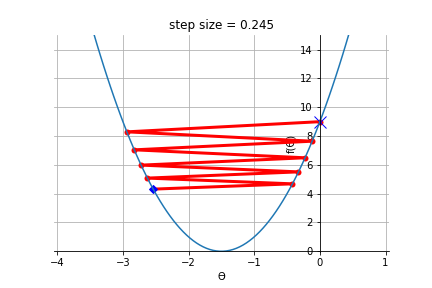
\includegraphics[width=70mm,scale=0.5]{images/gradient_descent_images/oscillate.png}
            \end{figure}
            
            We overshoot our target, and then have to take another step that \textbf{undoes} most of what happened in the previous step. So, we waste a lot of time correcting the last step.
                \note{For example, our first two steps land us in almost the same place we started!}
                
            This can significantly \textbf{slow} down how quickly we converge.
                
            \begin{figure}[H]
                \centering
                    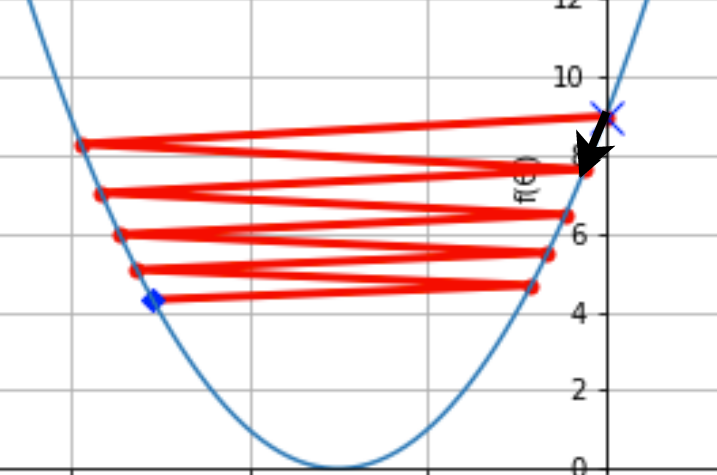
\includegraphics[width=70mm,scale=0.5]{images/nn_2_images/oscillate_zoom.png}
                
                \caption*{The black arrow shows the combined effect of our first two steps: almost nothing!}
            \end{figure}
            
            We don't want to waste time, so we want to remove the "part" of the gradient that is likely to \textbf{cancel} out. 
            
            The \textbf{next} gradient cancels out some of the previous. Our first two steps add up, or "\textbf{average} out" to a small improvement.
            
            If our steps are effectively "averaging", we'll speed up that process: we'll average together the gradients \textit{before} taking our step!
                \note{This means we can take a bigger step in a direction we won't have to cancel!}\\
                
            \begin{concept}
                Since our gradient descent steps \gren{combine} to give us our new model, we can think of them as adding, or "\purp{averaging}" to a more accurate improvement.
            \end{concept}
            
                \note{The only real difference between adding and averaging is whether we divide by the number of terms.}
            
            When our function \textbf{oscillates}, we get the same pattern \textbf{multiple} times: past steps indicate the sort of pattern we'll see in \textbf{future} steps. 
            
            So, we'll average our current gradient with past gradients: that way, the \textbf{component} that gets cancelled out is \textbf{removed}, and we won't have to undo our mistake over and over.\\
            
            \begin{concept}
                \vocab{Oscillation} causes us to move back and forth over the same region \purp{multiple} times, where each step mostly \gren{cancels} out the last.
                
                One solution is to \purp{average out} multiple of our gradients: the part that is "\gren{cancelled} out" should be eliminated by the average.
                
                So, we average our \gren{past} gradients (past oscillation) with our \gren{current} gradient, so we move in a more \purp{efficient} direction, speeding up our algorithm.
            \end{concept}
            
            Another way to think about it: when we \textbf{average} out our current and previous gradient, we're cancelling out what they "\textbf{disagree}" on, and keeping what they \textbf{agree} on.
            
            So, we're taking a step in the direction that multiple gradients agree will \textbf{improve} our model!
            
        
        \subsecdiv
            
        \subsubsection{Weighted averages}
        
            We could naively average all of our gradients \gren{equally}. But, this would be a bad idea:
            
            \begin{itemize}
                \item It doesn't give you as much control of the algorithm: what if we care more about the \textbf{present} gradient, than the previous one?
                \item Gradients further in the \purp{past} are \textbf{less likely} to matter: we've moved further away from those positions.
                    \begin{itemize}
                        \item We also need to \textbf{scale} down past terms, so they don't take up most of the average.
                            \note{If you're averaging 100 terms, and you add one more... it's not going to change much.}
                    \end{itemize}
            \end{itemize}
            
            The first problem is easy to solve: we'll \textbf{weigh} each of our terms differently.\\
            
            \begin{concept}
                A \vocab{weighted average} is used when we want some terms to affect our \purp{average} more than others.
                
                We represent this with \gren{weights}: each weight represents the \purp{proportion} of our average from that term.
                
                \begin{equation*}
                    \text{Weighted Average} =
                    x_1w_1 + x_2w_2 + \dots + x_nw_n
                \end{equation*}
            \end{concept}

                \note{These weights are \orgg{separate} from the weights inside our neural network.

                \phantom{}
                
                They do, however, represent the same type of concept: the NN weights scale the \gren{input}, while these weights scale the \purp{gradients}.}
            
            \miniex If $w_1=\red{.6}$, that means \red{60\%} of the average comes from $x_1$.
            
            Note that, since we're talking about \textbf{proportions}, they need to \orgg{sum to 1}: it wouldn't make sense to have more than 100\% of the average.
            
            At each time step, we're adding one new gradient: the \textbf{present} one.
            
            We'll simplify our average to those two terms: the \textbf{present} gradient, versus all the \textbf{past} gradients.
            
            \begin{itemize}
                \item We represent the importance (\textbf{weight}) of our \redd{past} gradients using the variable $\red{\gamma}$.
                
                \item We want the two terms to add to 1: so, the importance of \vocab{current} gradient is $\blu{1-\gamma}$.
            \end{itemize}
            
            \begin{equation}
                \overbrace{
                    A_t 
                }^{\text{Average}}
                =
                \overbrace{
                    \red{\gamma} G_{t-1}
                }^{\text{Old gradients}}
                + \;\;
                \overbrace{
                    \blu{(1-\gamma)} g_{t}
                }^{\text{New gradient}}
            \end{equation}
            
            Now, we have \textbf{control} over how much the present or past gradient matters: we just have to adjust $\gamma$. 
            
        \subsecdiv
        
        \subsubsection{Running Average}
        
            We still have some work to do: first, we haven't made it clear how we're incorporating our old gradients: we lumped them into one term.
            
            Let's try building up from $t=1$. We'll assume our previous gradients are 0, for simplicity.
            
            \begin{equation}
                A_0=g_0=0
            \end{equation}
            
            Our first step will average this with our \textbf{first} gradient:
            
            \begin{equation}
                A_1 
                =  
                \red{\gamma} g_0 \;\;+\;\; \blu{(1-\gamma)} g_1
            \end{equation}
            
            Simplifying to:
            
            \begin{equation}
                A_1 =  \blu{(1-\gamma)} g_1
            \end{equation}
            
            What about our second step? 
            
            \begin{equation}
                A_2
                =
                \overbrace{
                    \red{\gamma} G_{t-1}
                }^{\text{Old gradients}}
                + \;\;
                \blu{(1-\gamma)} g_2
            \end{equation}
            
            We \textit{could} just plug in $g_1$. But, $A_1$ contains the information about our first gradient $g_1$, \textbf{and} the gradient before it, $g_0$.
            
            \begin{equation}
                A_2
                =
                \overbrace{
                    \red{\gamma} A_1
                }^{\text{Contains $g_1$, $g_0$}}
                + \;\;
                \blu{(1-\gamma)} g_2
            \end{equation}
            
            We can repeat this process:
            
            \begin{equation}
                A_3 = 
                \overbrace{
                    \red{\gamma} A_{2}
                }^{\text{Contains $g_2$,$g_1$, $g_0$}}
                + \;\;
                \overbrace{
                    \blu{(1-\gamma)} g_3
                }^{\text{New gradient}}
            \end{equation}

            And so, we've created a general way to \textbf{average} as our program \textbf{runs} through different gradients.

            \begin{equation}
                A_t \;\;=\;\; 
                \gamma A_{t-1} \;\;+\;\; 
                (1-\gamma) g_t
            \end{equation}

            To allow more flexibility, we'll allow $\gamma$ to \orgg{vary in time}, as $\gamma_t$.
            
            \begin{equation}
                A_t \;\;=\;\; 
                \org{\gamma_t} A_{t-1} \;\;+\;\; 
                (1-\org{\gamma_t}) a_t
            \end{equation}

            \begin{itemize}
                \item We call this a \textbf{running average}.\\
            \end{itemize}

            \begin{definition}
                A \vocab{running average} is a way to average past data with present data \purp{smoothly}.

                Our \gren{initial} value for the average is typically zero:

                \begin{equation*}
                    A_0=0
                \end{equation*}

                Then, we begin introducing \orgg{new} data points.
                
                \begin{itemize}
                    \item You use the parameter $\gamma_t$ to indicate how much you want to prioritize \gren{past data}.
                    \item Thus, $1-\gamma_t$ indicates the value of \purp{new data}.
                \end{itemize}

                \begin{equation*}
                    \overbrace{
                        A_t 
                    }^{\text{Average}}
                    \;\;=\;\;
                    \overbrace{
                        \red{\gamma_t} A_{t-1}
                    }^{\text{Old gradients}}
                    \;\;+\;\; 
                    \overbrace{
                        \blu{(1-\gamma_t)} g_{t}
                    }^{\text{New gradient}}
                \end{equation*}

                \subsecdiv

                \begin{itemize}
                    \item Note that instead of $\gamma$, we write $\gamma_t$: this "discount factor" can vary with time.

                \end{itemize}

                
            \end{definition}

            \phantom{}

            \begin{clarification}
                This is technically only one kind of \orgg{running average}: here, we use an "\vocab{exponential moving average}". 

                There are different ways to average past data points, with different \purp{weighting} schemes.
                    
                    \begin{itemize}
                        \item For example, you could do a "\gren{simple moving average}", where you average equally over the last $n$ data points.
                    \end{itemize}
            \end{clarification}

        \subsubsection{Running Averages: The Distant Past}

            So, how does this "running average" approach affect our different data points, further in the past? Let's find out.

            \subsecdiv

            For simplicity, let's assume $\gamma_t=\gamma$: it's a \gren{constant}.

            \begin{equation}
                A_t 
                =
                \red{\gamma} \grn{A_{t-1}}
                + 
                \blu{(1-\gamma)} g_{t}
            \end{equation}

            We can expand $A_{t-1}$ to see further in the past:

            \begin{equation}
                A_t 
                =
                \red{\gamma} 
                    \Big(\red{\gamma} \grn{A_{t-2}}
                    + 
                    \blu{(1-\gamma)} g_{t-1}
                \Big)
                + 
                \blu{(1-\gamma)} g_{t}
            \end{equation}

            And even further: 
                \note{This is starting to get messy: don't worry if it's hard to read.}
            

            \begin{equation}
                A_t 
                =
                \red{\gamma} 
                \Bigg(\red{\gamma} 
                    \Big(
                        \red{\gamma} \grn{A_{t-3}}
                        + 
                        \blu{(1-\gamma)} g_{t-2}
                    \Big)
                    + 
                    \blu{(1-\gamma)} g_{t-1}
                \Bigg)
                + 
                \blu{(1-\gamma)} g_{t}
            \end{equation}

            Let's rewrite this.

            \begin{equation}
                \red{\gamma}^3 \grn{A_{t-3}}  \;\;+\;\; 
                \red{\gamma}^2\blu{(1-\gamma)} g_{t-2} \;\;+\;\;
                \red{\gamma}\blu{(1-\gamma)} g_{t-1} \;\;+\;\; 
                \blu{(1-\gamma)} g_{t}
            \end{equation}

            \subsecdiv

            We see a "stacking" effect for $\gamma$: 
            
            \begin{itemize}
                \item We only partly include our newest data point: we scale it by $1-\gamma$, to make room for the past.

                \begin{equation}
                    \blu{(1-\gamma)} g_{t}
                \end{equation}
                
                \item But if your gradient is 1 time unit in the past, we apply $\gamma$ \orgg{once}, "forgetting" some more of that gradient.

                \begin{equation}
                    \red{\gamma}\blu{(1-\gamma)} g_{t-1}
                \end{equation}

                \item But if your gradient is 2 units in the past, we apply $\gamma$ \orgg{twice}: we've "forgotten" some of it twice.

                \begin{equation}
                    \red{\gamma}^2\blu{(1-\gamma)} g_{t-2}
                \end{equation}
            \end{itemize}

            Each time we do an average, we scale down our older data points by $\gamma$. So, the further in the past, the less effect they have.

            \begin{itemize}
                \item This is exactly the kind of design we wanted!\\
            \end{itemize}

            \begin{concept}
                A \purp{running average} tends to pay less attention to data further in the \gren{past}.

                \begin{itemize}
                    \item In general, if you are $k$ time units in the past, we apply a factor of \red{$\gamma^k$}.
                \end{itemize}

                Because $\gamma<1$, this \orgg{exponentially} decays to 0.

                \subsecdiv

                If we want to fully expand $A_t$, it's easiest to use a sum:

                \begin{equation*}
                    A_T = \sum_{t=0}^T \red{\gamma^{(T-t)}} \cdot \blu{(1-\gamma)} \cdot g_t
                \end{equation*}
            \end{concept}
            You can compare this formulation against what we computed above.

            \subsecdiv
            
        \subsubsection{Momentum}

            Applying a running average to our gradients gives us \purp{momentum}.

            \begin{itemize}
                \item This analogy to \textbf{physics} represents how our point "moves" through the \purp{weight space}, to optimize $J$.
                    \note{Gradient descent adjusts our weights: we go from one list of weights, to another. That's why we say we're moving through the "weight space".

                    \phantom{}
                    
                    Because our hypothesis is determined by our weights, this is also a "hypothesis space".}
                    
                \item The gradient gives us a "direction" of motion. So, our \gren{momentum} represents the direction we were "already moving": the \gren{previous} averaged gradient.
            \end{itemize}

            We use $M$ to represent the "averaged gradient" that we use to move. Our initial momentum is 0:

            \begin{equation}
                M_0=0
            \end{equation}

            And we want to average our current gradient with past gradients:

            \begin{equation}
                M_t 
                \;\;=\;\;
                \red{\gamma} \grn{M_{t-1}}
                \;\;+\;\; 
                \blu{(1-\gamma)} g_{t}
            \end{equation}

            What is our \purp{past} gradient $g_t$? Well, we want to use $W$ to modify $J$: $\pderiv{J}{W}$, or $\nabla_W J$.

            And we're moving through the \gren{weight space}, so our input to the gradient is the previous set of weights, $W_{t-1}$.

            \begin{equation}
                g_{t} = \nabla_W J (W_{t-1})
            \end{equation}

            And finally, $M_t$, our "averaged gradient", determines how we move.

            \begin{equation}
                W_t \;\;=\;\; W_{t-1} \;\;-\;\; \eta M_t
            \end{equation}

            \begin{definition}
                \vocab{Momentum} is a technique for gradient descent where we do a \gren{running average} between our current gradient, and our older gradients.

                This approach reduces \purp{oscillation}, and thus aims to improve the speed of convergence for our models.

                \begin{itemize}
                    \item Our initial "momentum" (averaged gradient) is \orgg{0}.
                    \item The amount we value new data is given by $\red{\gamma_t}$.
                    \item Old data is scaled by $\blu{1-\gamma_t}$.
                \end{itemize}

                \begin{equation*}
                    \begin{gathered}
                        M_0=0 \\
                        M_t 
                        \;\;=\;\;
                        \overbrace{
                            \red{\gamma_t} M_{t-1}
                        }^{\text{Old gradients}}
                        \;\;+\;\; 
                        \overbrace{
                            \blu{(1-\gamma_t)} \nabla_W J (W_{t-1})
                        }^{\text{New gradient}}
                    \end{gathered}
                \end{equation*}

                We use this momentum to take our step:

                \begin{equation*}
                    W_t \;\;=\;\; W_{t-1} \;\;-\;\; \eta \grn{M_t}
                \end{equation*}
                
                \subsecdiv

                This approach puts more emphasis on newer data points, and less on older ones.
            \end{definition}

            \miniex We can see this "dampened oscillation" in action below:

            \begin{figure}[H]
                \centering
                    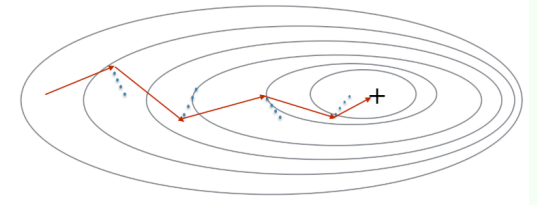
\includegraphics[width=70mm,scale=0.5]{images/nn_2_images/momentum.png}
                
                \caption*{The blue lines indicate the more "severe" path that we would've taken with normal gradient descent. the orange line is the line we take with momentum. }
            \end{figure}

            Notice that generally, the orange path is closer to correct! We still oscillate somewhat, but much less than we would have otherwise.

            \pagebreak

            
            

            

    \subsection{Adadelta}    

        \subsubsection{Per-weight step sizes}

            Earlier, we discussed creating \textbf{separate} step sizes for different weights in our network:
    
            \begin{itemize}
                \item Different weights could have different \gren{sensitivities}: one weight could have a much larger/smaller impact on $J$, based on \textbf{structure}.
    
                \item We already have the challenge of figuring out what \textbf{step sizes} cause \purp{slow convergence/divergence}: it would be even harder to find a step size that fit \textbf{all} of our weights, at the same time.
            \end{itemize}
    
            So, instead, we decided that each weight gets its \textbf{own step size}. 

            \begin{itemize}
                \item But, we never elaborated on \textbf{how} we compute that (adjustable) step size.\\
            \end{itemize}

            \begin{notation}
                Our base step size is indicated as $\eta$. 
                
                We'll call the \orgg{modified} step size for weight $j$, $\eta_j$.
            \end{notation}
            

        \subsubsection{Scaling}

            Our goal now, is to come up with a \orgg{systematic} way to \orgg{assign step sizes}. This allows us to \textbf{adjust}, rather than run our whole gradient descent with a "bad" step size.
                \note{So, we have less of a problem if we choose $\eta$ poorly.}

            Why do we adjust our step size? To avoid slow convergence, oscillation, or divergence.

            \begin{itemize}
                \item We might expect \purp{slow convergence} if the derivative is too \purp{small}: we carefully take small steps, but we aren't having much of an impact on $J$.

                    \begin{itemize}
                        \item Across this "flatter" region of the surface, in one direction, we might expect it to be safer to move further.
                    \end{itemize}

                \item We might expect \gren{divergence} or \gren{oscillation} if the derivative is too \gren{large}.
                    \begin{itemize}
                        \item We might end up "missing" possible solutions/local minima by \textbf{overshooting} them.
                        \item So, "steeper" regions might be riskier.
                    \end{itemize}
            \end{itemize}

            \begin{concept}
                Our goal is to \orgg{scale} our step size, so that it \textbf{adapts} to the situation:

                \begin{itemize}
                    \item We want to \purp{shrink} our step for \purp{large} gradients
                    \item We want to \gren{increase} our step for \gren{small} gradients
                \end{itemize}

                And we're interested in the \orgg{magnitude} of these gradients.
            \end{concept}


            This sort of behavior is easily captured by including a factor of $1/\norm{g_t}$. However, this has a smoothness problem: so, we'll use $1/\norm{g_t}^2$ instead.

            Though, we need to keep it separate for each of our data points.\\

            \begin{notation}
                The gradient for \vocab{weight $j$} at \redd{time $t$} is given as 

                \begin{equation*}
                    g_{\red{t},\blu{j}} = \nabla_W J(W_{\red{t-1}})_{\blu{j}}
                \end{equation*}

                Note the double-subscript.

                \subsecdiv

                \begin{itemize}
                    \item By isolating weight $j$, we have a constant, not a vector.
                \end{itemize}
            \end{notation}

            We can now write our gradient update rule:

            \begin{equation}
                W_{\red{t},\blu{j}} \;\;=\;\; 
                W_{\red{t-1},\blu{j}} \;\;-\;\; 
                \eta_{\blu{j}} \cdot g_{\red{t},\blu{j}}
            \end{equation}

            And we're currently using the step size
                \note{Don't save this equation! It isn't our final formula.}

            \begin{equation}
                \eta_{\blu{j}} = \frac{\eta}{g_{\red{t},\blu{j}}^2}
            \end{equation}

        \subsubsection{Averaging}

            But, we don't necessarily know how "steep" our region \textbf{generally} is, based on the current gradient $g_t$. $g_t$ only gives us \textbf{one point} in space.
            
            It would be helpful to include information from the \textbf{past}: we'll be re-using the \textbf{weighted average}, once again.
                \note{Once again, it's helpful that the weighted average gradually "forgets" older information: we care less about gradients which are "further" from the present.}

            \begin{equation*}
                G_t \;\;=\;\; 
                \gamma G_{t-1} \;\;+\;\; 
                (1-\gamma) g_t^2 
                \qquad \qquad \text{(Maybe?)}
            \end{equation*}

            \begin{itemize}
                \item Note that we're averaging the \textbf{squared} magnitude.
            \end{itemize}
            
            Technically this is still \textbf{incorrect}: we need the $j$ notation.
                \note{It's incorrect because $g_t$ is a vector: we can't square it directly, we have to square its magnitude.}

            \begin{equation*}
                G_{\red{t},\blu{j}} \;\;=\;\; 
                \gamma G_{\red{t-1},\blu{j}} \;\;+\;\; 
                (1-\gamma) g_{\red{t},\blu{j}}^2 \qquad \qquad 
                \text{(Fixed!)}
            \end{equation*}

        \subsubsection{Division by zero}

            There's a problem with our weight adjustment:

            \begin{equation}
                \eta_j = \frac{\eta}{G_{\red{t},\blu{j}}}
            \end{equation}

            What happens if the denominator is near zero? It'll explode to a huge number! And at zero, it's undefined.

            To solve this, we'll add a very small constant, $\epsilon$.
                \note{We won't prescribe any particular choice of $\epsilon$ here.}

                \begin{equation}
                    \eta_j = \frac{\eta}{G_{\red{t},\blu{j}}+\epsilon}
                \end{equation}

            Now, our scaling factor will never be bigger than $1/\epsilon$.

        \subsubsection{Square root}

            One last concern, to wrap up: currently, we're diving by the \textbf{squared} gradient. This is actually somewhat overkill. 
            
            Remember that our goal is to do the following operation:

            \begin{equation}
                W_{\red{t},\blu{j}} = W_{\red{t-1},\blu{j}}  \;\;-\;\; 
                \underbrace{
                    \eta_{\blu{j}} \cdot g_{\red{t},\blu{j}}
                }_{\text{Update}}
            \end{equation}

            With our current formula, our update has 
            
            \begin{itemize}
                \item a factor of $g_{t,j}$ in the \textbf{numerator}
                \item from $\eta_j$, a factor proportional to $g_{t,j}^2$ in the \textbf{denominator} 
            \end{itemize}

            This is "scaling" our gradient by more than we want to. So, we'll take the \textbf{square root} of the denominator.
                \note{Our goal is to make the scales of different axes more similar, not to neglect dimensions with high gradient (high effect on loss)}

            \begin{equation}
                \eta_j = \frac{\eta}{ \sqrt{G_{\red{t},\blu{j}}+\epsilon} }
            \end{equation}

            This is the completed form of our \textbf{adadelta step size rule!}

            \begin{definition}
                \vocab{Adadelta} is a technique for \redd{adaptive step size}, which:

                \begin{itemize}
                    \item \purp{Decreases} step size in dimensions with a history of \purp{high-magnitude} gradients
                    \item \gren{Increases} step size in dimensions with a history of \gren{low-magnitude} gradients
                \end{itemize}

                Suppose our gradient for weight $W_j$ at time $t$ is represented by

                \begin{equation*}
                    g_{t,j} = \nabla_{W}J(W_{t-1})_j
                \end{equation*}

                    \subsecdiv

                This is accomplished by \orgg{scaling} the step size $\eta$ to create $\eta_j$:

                \begin{equation*}
                    \eta_j = \frac{\eta}{ \sqrt{G_{\red{t},\blu{j}}+\epsilon} }
                \end{equation*}

                Where $G_{t,j}$ is a "\redd{running average}" of the previous gradients for weight $W_j$.

                \begin{equation*}  
                    \begin{gathered}
                        G_{\red{0},\blu{j}} = 0 \\
                        G_{\red{t},\blu{j}} \;\;=\;\; 
                        \gamma G_{\red{t-1},\blu{j}} \;\;+\;\;
                        (1-\gamma) g_{\red{t},\blu{j}}^2
                    \end{gathered}
                \end{equation*}

                So, our completed gradient descent rule takes the form:

                \begin{equation*}
                    W_{\red{t},\blu{j}} \;\;=\;\; 
                    W_{\red{t-1},\blu{j}}  \;\;-\;\; 
                    \frac{\eta}{ \sqrt{G_{\red{t},\blu{j}}+\epsilon} } \cdot g_{\red{t},\blu{j}}
                \end{equation*}
                
            \end{definition}

        \subsubsection{Sparse Data}

            One major advantage of adadelta is its use for \orgg{sparse datasets}, where many variables only show up in a small percentage of the data.

            \begin{itemize}
                \item If a variable is much less frequent, then the weighted average $G_t$ will be much smaller.
                \item So, when those data points \textbf{do} appear, the step size is much larger.
            \end{itemize}

            This allows our model to learn more from variables that don't show up as frequently.\\

            \begin{concept}
                \vocab{Adadelta} often works well with \purp{sparse data}: datasets where many variables rarely show up as non-zero.

                The step sizes for these variables become much larger, so our model can learn more from less-common information.
            \end{concept}

            However, this can run the risk of paying attention to variables that are sparse, but \textbf{not} especially meaningful. 
            
            \begin{itemize}
                \item It's important to choose your variables carefully, so the model doesn't "learn" from noise.
            \end{itemize}

        \subsubsection{Adagrad}

            Originally, adadelta derives from a \textbf{simpler} method, known as \vocab{adagrad}, or "adaptive gradient".

            \begin{itemize}
                \item The main difference with this approach is, rather than find the \textbf{weighted average} $G_t$, we simply \textbf{sum} the previous gradients.
            \end{itemize}

            The main problem with this approach is that, over time, $G_t$ becomes too \textbf{large}. So, our step size becomes too small, and our algorithm slows down.

            By averaging, we don't run into this problem of $G_t$ "accumulating": older data is gradually \textbf{forgotten}.

    \pagebreak
    \subsection{Adam}

        Momentum and Adadelta both bring some benefits:

        \begin{itemize}
            \item \purp{Momentum} averages our current gradient with \purp{previous gradients}, to reduce \textbf{oscillation} and make a more direct path to the solution.
            
            \item \gren{Adadelta} modifies our \gren{step sizes}: it takes smaller steps in directions of high gradient (reduce overshooting) and takes bigger steps in directions of low gradient (converge faster).
        \end{itemize}

        There's nothing structurally incompatible between them. So, why not incorporate both?

        \begin{itemize}
            \item This combination is called \vocab{Adam}: it has become the most popular way to handle step sizes in neural networks.\\
        \end{itemize}

        \begin{concept}
            \vocab{Adam} integrates the techniques of both \purp{momentum} and \gren{adadelta}.
        \end{concept}

        \subsecdiv

        \subsubsection{Momentum and Adadelta}

            We used two different \textbf{running averages}, both using $\gamma$ for their "\textbf{discount factor}": how much we discount the effect of older data.
                \note{It's "discounting", or reducing the effect of older data, because $\gamma<1$.}
    
            \begin{itemize}
                \item We'll replace $\gamma$ with $B_1$ (momentum) and $B_2$ (adadelta).\\
            \end{itemize}

            \begin{notation}
                In the adam algorithm, $B_1$ and $B_2$ are \redd{discount factors} replacing $\gamma$ from momentum and adadelta.
            \end{notation}
    
            We use the same notation for gradients:
    
            \begin{equation}
                g_{t,j} = \nabla_W J(W_{t-1})_j
            \end{equation}
    
            First, we'll keep track of our\textbf{ averaged gradient}, $m_{t,j}$. This will be the \textbf{direction} we plan to move.

            \begin{equation}
                \blu{m_{t,j}} \;\;=\;\; 
                B_1 \blu{m_{t-1,j}} \;\;+\;\; 
                (1-B_1) \blu{ g_{t,j} }
            \end{equation}

            Then, we'll keep track of the \textbf{average squared gradient}, $v_{t,j}$. This will tell us whether to scale up/down our \textbf{step size} on each variable.

            \begin{equation}
                \red{v_{t,j}} \;\;=\;\; 
                B_2 \red{v_{t-1,j}} \;\;+\;\; 
                (1-B_2) \red{ g_{t,j}^2 }
            \end{equation}

            We can combine these into our equation, the way you use momentum and adadelta:

            \begin{equation}
                W_{t,j} \;\;=\;\; 
                W_{t-1,j}  \;\;-\;\; 
                \frac{\eta}{ \sqrt{\red{v_{t,j}}+\epsilon} } \cdot \blu{m_{t,j}}
            \end{equation}

            We're not quite done yet, though.

        \subsubsection{Normalization}

            There's one issue with our running average, that we should address.

            Suppose we have a sequence of numbers:

            \begin{equation}
                [1,1,1]
            \end{equation}

            What's the running average of this sequence of numbers, with $\gamma=.1$? You'd expect it to be 1 for all elements, right?

            \begin{itemize}
                \item We start with $a_0=0$.
            \end{itemize}

            \begin{equation}
                \begin{gathered}
                    a_1 = .1*0 + .9*1 = \org{.9} \\
                    a_2 = .1*.9+ .9*1 = \org{.99} \\
                    a_3 = .1*.99+ .9*1 = \org{.999}
                \end{gathered}
            \end{equation}

            It turns out not to be true! Why is that?

            Because of our initial term, $a_0$: it has nothing to do with the data. Because it'll always be 0, it \textbf{deflates} the value of all the remaining averages.

            How much does it deflate the average? Well, let's consider the general equation:

            \begin{equation}
                A_T = \sum_{t=0}^T \red{\gamma^{(T-t)}} \blu{(1-\gamma)^t} g_t
            \end{equation}

            What "fraction" of the total is missing, thanks to $A_0=0$? 
            
            \begin{itemize}
                \item Well, all of our weighted terms $\red{\gamma^{(T-t)}} \blu{(1-\gamma)^t}$ should add up to 1: each one represents the "percent/fraction" of the average which comes from that $g_t$ term.
            \end{itemize}

            $A_0$ matches $t=0$, so we find:

            \begin{equation}
                A_T = \overbrace{ A_0 \red{\gamma^T}}^{A_0=0} + 
                \sum_{t=1}^T \red{\gamma^{(T-t)}} \blu{(1-\gamma)^t} g_t
            \end{equation}

            So, out of our total $1$, or 100\%, we're missing $\gamma^T$.

            \begin{itemize}
                \item Our new total is $1-\gamma^T$.

                \item In order to correct for the "zeroed out" part of our average, we multiply by

                \begin{equation}
                    \frac{\text{Desired total}}{\text{Real total}}=\frac{1}{1-\gamma^T}
                \end{equation}
            \end{itemize}

            \begin{concept}
                We've chosen $A_0=0$: this is \orgg{unrelated} to our real data. 
                
                As a result, $A_t$ doesn't accurately reflect our weighted average: it's slightly \gren{smaller}.

                \begin{itemize}
                    \item $A_0$ is "included" as a 0, even though it's not a \redd{real} data point.
                    \item So, whatever \purp{percent} of our data is represented by $A_0$, is "falsely empty".
                \end{itemize}

                $A_0$ is scaled by $\red{\gamma^t}$, so that's the amount \purp{removed} from our "true" weighted average.

                The "real" weighted average, that ignores $A_0$, has to un-do the deflation caused by including fake, starting data:

                \begin{equation*}
                    \widehat{A}_t = A_t \cdot \frac{1}{1-\gamma^t}
                \end{equation*}
            \end{concept}

            We'll make this correction for our running averages:

            \begin{equation}
                \begin{gathered}
                    \widehat{m}_{t,j} = \frac{m_{t,j}}{1-B_1^t} \\
                    \widehat{v}_{t,j} = \frac{v_{t,j}}{1-B_2^t}
                \end{gathered}
            \end{equation}

        \subsubsection{Adam}

            Now, we have our complete equation for adam:\\

            \begin{definition}
                \vocab{Adam} is a technique for improving \orgg{gradient descent} that integrates two other techniques. Our computed gradient is given as 

                \begin{equation*}
                    g_{t,j} = \nabla_{W}J(W_{t-1})_j
                \end{equation*}

                \begin{itemize}
                    \item \purp{Momentum} averages our previous gradients with our current one, to reduce oscillation and get a "averaged" view of data. $B_1$ gives the weight of old data.

                        \begin{equation*}
                            \begin{gathered}
                                m_{0,j} = 0 \qquad \qquad
                            \blu{m_{t,j}} \;=\; B_1 \blu{m_{t-1,j}} \;+\; (1-B_1) \blu{ g_{t,j} }
                            \end{gathered}
                        \end{equation*}

                    \item \gren{Adadelta} estimates how "steep" our gradient has been recently, and uses it to adjust our step size, for better convergence. $B_2$ gives the weight of old data.

                            \begin{equation*}
                                \begin{gathered}
                                    v_{0,j} = 0 \qquad \qquad
                                    \red{v_{t,j}} \;=\; B_2 \red{m_{t-1,j}} \;+\; (1-B_2) \red{ g_{t,j}^2 }
                                \end{gathered}
                            \end{equation*}
                        \end{itemize}

                We include a \textbf{correction} factor for the zeroed initial conditions: $m_0=v_0=0$.

                \begin{equation*}
                    \widehat{\blu{m}}_{t,j} = \frac{\blu{m}_{t,j}}{1-B_1^t}
                    \qquad \qquad 
                    \widehat{\red{v}}_{t,j} = \frac{\red{v}_{t,j}}{1-B_2^t}
                \end{equation*}

                Finally, our update rule takes the form:

                \begin{equation*}
                    W_{t,j} = W_{t-1,j}  
                        \;\;-\;\; 
                    \frac{\eta}{ \sqrt{\red{\widehat{v}_{t,j}}+\epsilon} } \cdot \blu{\widehat{m}_{t,j}}
                \end{equation*}
            \end{definition}

            Impressively, adam is not very sensitive to the initial conditions for $\epsilon$, $B_1$ and $B_2$.
                \note{It's able to "self-correct" its step sizes and gradient based on data.}

            To implement this for NNs, we just need to keep track of each value, for each weight. If you do it systematically, this is easier than it sounds.
            




\pagebreak

\section{Regularization}

    Something we haven't discussed in a while, that we might investigate, is \orgg{regularization}: techniques against overfitting.

    \begin{itemize}
        \item We teach our model using "training data", which, by chance, may not perfectly reflect the \textbf{true} distribution.
    \end{itemize}

    We want to apply this to our modern, deep neural networks, with their huge number of \textbf{parameters}, and huge amount of \textbf{data}. And yet...
    
    These modern neural nets \gren{don't} tend to have as much problem with \purp{overfitting}, and we're not sure \textbf{why}!

    Regardless, we do still have \textit{some} methods for regularization: this will be our focus for the rest of this chapter.

    \subsection{Methods related to ridge regression}

        We'll start with methods that we can bring back from classic ridge regression.

        \subsubsection{Early Stopping}

            One component built into our learning algorithm for regression is \purp{early stopping}: we check if the model is still making \textbf{progress}. If it isn't, then we \textbf{stop} training.

            \begin{itemize}
                \item The longer we train our model, the more time it has to "\textbf{memorize}" the exact structure of our training data: including \textbf{noise}.
            \end{itemize}

            We would typically either measure the size of the \gren{gradient}, or the change in the \purp{loss}. If either was small, then we might be in a local minimum: we've finished training.

            \subsecdiv

            So, we do the same here: after a period of training (over the whole dataset, called an \vocab{epoch}), we measure the \textbf{loss} on a validation set.

            \begin{itemize}
                \item If the loss stops decreasing, or begins \orgg{increasing}, our model is probably \textbf{overfitting}. We \redd{stop early}.
            \end{itemize}

            Then, you return the weights with the lowest error.\\

            \begin{definition}
                An \vocab{epoch} is the time frame during which your model sees your whole \purp{training data} set, \orgg{once}.

                \subsecdiv

                With \vocab{early stopping}, you evaluate your model using your \purp{validation data}, computing the loss.

                \begin{itemize}
                    \item If the loss has decreased from the last epoch, you \gren{continue} training.
                    \item If the loss has stopped decreasing, or is increasing, you \redd{stop} training.
                \end{itemize}

                This continues until you've either run out of \textbf{epochs}, or you've met your \textbf{termination} condition, and stopped early.

                \subsecdiv

                \begin{itemize}
                    \item Note that sometimes, "epoch" just refers to how long you train before you check your loss.
                    \item In this case, it might be smaller than the whole dataset.
                \end{itemize}
            \end{definition}


            \subsubsection{Weight Decay}

                We can also use the same kind of regularization term that we used for linear regression: penalizing the \purp{squared magnitude}.

                \begin{itemize}
                    \item Starting with our loss function:
                        \begin{equation}
                            J_{loss} = \sum_{i = 1}^{n}
                                \mathcal{L}( \red{\text{NN}(x^{(i)})},\;\; \blu{y^{(i)}};\;\; \grn{W})
                        \end{equation}
                    \item And we penalize based on the square magnitude of our weights:
                        \begin{equation}
                            J = \lambda \norm{\grn{W}}^2 +
                                J_{loss}
                        \end{equation}
                \end{itemize}

            If we take the gradient, we get:

            \begin{equation}
                \nabla_W J = 2\lambda \grn{W} + 
                    \nabla_W J_{loss}
            \end{equation}

            Let's see how the regularization affects our step:

            \begin{equation}
                \grn{W_t} = 
                \grn{W_{t-1}} - 
                \eta \Big( 2\lambda \norm{\grn{W_{t-1}}} + 
                     \nabla_W J_{loss} \Big)
            \end{equation}

            It directly subtracts from our weight, \orgg{decaying} it.

            \begin{equation}
                \grn{W_t} = 
                \grn{W_{t-1}} \Big( \org{ 1 -  2\lambda \eta } \Big)  - 
                     \eta \nabla_W J_{loss} 
            \end{equation}

            Thus, we call it \textbf{weight decay}.\\

            \begin{concept}
                When we apply \purp{square magnitude} regularization to the weights of a neural network, we call it \vocab{weight decay}.

                \begin{equation*}
                    J_{reg} = J_{loss} + \lambda \norm{W}^2
                \end{equation*}

                That's because, when you take the gradient, it directly subtracts from weight $W$, causing it to \orgg{decay} by a factor of $(1-2\lambda \eta)$.

                \begin{equation*}
                    \grn{W_t} = 
                    \grn{W_{t-1}} \Big( \org{ 1 -  2\lambda \eta } \Big)  - 
                         \eta \nabla_W J_{loss} 
                \end{equation*}
            \end{concept}

        \subsubsection{Perturbation}

            One last way to reduce overfitting is to add some \orgg{random noise} to our data: each variable has a small, random number added to it.

            This value is typically \purp{zero-mean} and \gren{normally distributed}:

            \begin{itemize}
                \item Zero-mean: it has 0 effect, on average, so it doesn't bias the data high or low.
                \item Normally distributed: the noise is \textbf{symmetric}: +2 and -2 are equally likely.
                    \note{The "normal distribution" contains more information than that, but the symmetry is important.}
            \end{itemize}

            How large the noise is, depends on the chosen \textbf{variance}.
            
            This reduces overfitting, because if the data is slightly different each time you see it, it's harder to perfectly "memorize" the exact shape and structure.\\

            \begin{definition}
                \vocab{Perturbation} is a technique where you slightly modify your system.

                \begin{itemize}
                    \item In our case, we're \gren{randomly} adding small amount of \purp{noise} to our input data.
                \end{itemize}

                This makes it more difficult for the model to \orgg{overfit}, because the patterns aren't always exactly the same.

                \begin{itemize}
                    \item Only the "general", high-level patterns are preserved, each time you view the dataset.
                \end{itemize}
            \end{definition}

            Of course, if you perturb your data too strongly, you can miss real patterns. Your perturbations shouldn't be too large.

            

    \subsection{Dropout}

        We also have \textbf{structural} ways of dealing with overfitting. We discussed perturbing the \purp{dataset}, but we could, instead, perturb the \gren{model} itself!

        

        We do this by randomly \redd{removing} some weights from the neural network, and training. 

        \begin{itemize}
            \item Each weight has a probability $p$ of being "turned off": the \textbf{activation} is set to zero.

            \begin{equation}
                a^\ell_j=0
            \end{equation}

            \item Thus, that neuron's output is \textbf{ignored} by the next layer, and receives no training.

            \item At the next step, we remove a \textbf{different} random selection of weights. 
        \end{itemize}

        Because our model keeps changing slightly, it's harder to exactly \textbf{overfit} to the data.

        \subsecdiv

        This particular approach also addresses a \textbf{different} kind of overfitting:

        \begin{itemize}
            \item One model might heavily "rely" on a \textbf{small} number of neurons to make decisions.
            \item This makes our model less flexible, uses the weights less efficiently.
        \end{itemize}
        
        To solve this, we prevent the neural network from using some of these weights, \textbf{randomly}.

        Thus, the whole network "\textbf{shares}" some responsibility for  getting the right answer.\\

        \begin{definition}
            \vocab{Dropout} is a process where, at each training interval, you \orgg{randomly} "drop out", or de-activate, some of the weights in the network.

            \begin{itemize}
                \item Each neuron has probability $p$ of being turned off.
                \item These neurons have their \gren{activation} set to zero: $a^\ell_j=0$.
            \end{itemize}

            This process is designed to reduce \purp{overfitting}. As the network randomly changes, it's harder for it to perfectly match the data structure.

            \subsecdiv

            \begin{itemize}
                \item When the network is finished training, we multiply all the weights by $p$. Why?
            
                \item Because during training, only $p$ fraction of the neurons were active. We want to replicate that average activity level, even when we use all of our neurons.
            \end{itemize}

            

            \subsecdiv

            This process is also designed to create "collective responsibility" for your neurons. It prevents your network from relying on a small number of neurons to solve problems.

            It generally improves \orgg{robustness} against random variations in the data.
        \end{definition}

        

        \subsecdiv

        This approach has, in recent years, become somewhat less popular, for a couple reasons:

        \begin{itemize}
            \item Very \textbf{large} networks don't struggle as much with overfitting.
            
            \item CNNs tend not to benefit from this procedure, because of \textbf{weight-sharing}: the same weights are re-used in multiple places.
                \note{We'll discuss CNNs in our next chapter.}

            \item Like most ML techniques, their usefulness depends on the situation.
        \end{itemize}

        It still finds use in some smaller models, RNNs, etc.

        In many places, it has been replaced by \vocab{batch normalization}.

    \pagebreak

    \subsection{Batch Normalization}

        \subsubsection{Covariate Shift}

            Our last approach related to regularization was designed to handle a new type of problem we call \textbf{covariate shift}:
            
            When you run \textbf{gradient descent} on a neural network, you're adjusting the weights of all of our layers, at the \textbf{same time}.
    
            Let's focus on layer 1 and layer 2. By updating layer 1, we've changed the outputs it creates: the same $\ex{x}{i}$ now creates a different output, going from $a^1_{old}$ to $a^1_{new}$.
    
            But, this output is the \textbf{input} of layer 2.
            
            \begin{itemize}
                \item This means that layer 2 is now receiving \purp{different inputs} than it was before.
                    
                \item This is a problem: layer 2 just received training based on the \gren{old} inputs $a^1_{old}$!
            \end{itemize}
    
            This makes life a lot harder for our layer 2: not only is it learning to make better predictions, it also has to adjust for the change in layer 1. This is a form of \vocab{covariate shift}.\\
    
            \begin{definition}
                \vocab{Covariate shift} occurs when the distribution of input variables \purp{changes} over time. 
    
                \begin{itemize}
                    \item This can cause our original model to become inaccurate, or "outdated": it was trained on \purp{different} data.
                \end{itemize}
    
                \vocab{Internal covariate shift} occurs because of changes to the network itself.
                
                \begin{itemize}
                    \item The distribution of inputs to \gren{later layers} changes, because \gren{earlier layers} have changed through training.
                \end{itemize}
            \end{definition}
    
            \miniex If the weights in layer 1 all get smaller (as a side effect of correcting them), layer 2 may have to make all of its weights bigger to compensate.
            
            \begin{itemize}
                \item Our expectation is that this extra work would slow down training.
            \end{itemize}

        \subsubsection{Layer Normalization}

            So, we want to counter the problem of how the input to layer 2 \textbf{changes} based on layer 1's \textbf{learning}.

            \begin{itemize}
                \item But, at the same time, we don't want to \textbf{undo} the work that we did \textbf{training} layer 1.
                \item So, we want to preserve the information in layer 1, while making it easier to use.
            \end{itemize}

            In our example, we mentioned that the scale of the inputs might get larger: they all get bigger or smaller, at the same time.

            But, we often want to know what makes these inputs \textbf{different} from each other, so we can compare them: it's not helpful if all of them become larger/smaller.

            So, we'll \vocab{standardize} each of our mini-batches of data, between each layer:
                \note{This is exactly the same as when we standardized in the Feature Transformation chapter.}

            \begin{itemize}
                \item \purp{Subtracting the mean}: we take the mean of the mini-batch input, and subtract it from each data point. So, our standardized data is always centered at 0.

                \item \gren{Dividing by standard deviation}: we compute how "spread out" the data is, and scale by that factor. Our standardized data is always the same amount "spread out".
            \end{itemize}

            We repeat this process in between each layer of our network. Each layer currently receives a set of inputs with mean 0, standard deviation 1. No matter how the earlier layers change.
                \note{Below, we exclude the $\ell$ superscript in $z^\ell$, $\mu^\ell$, $\sigma^\ell$, and $n^\ell$ for readability.}\\

            For now, we'll apply this to the pre-activation $Z$.\\

            \begin{concept}
                In order to deal with \vocab{internal covariate shift}, we'll take each mini-batch of $k$ \gren{pre-activations} to each \gren{layer} (pre-activation, not true "input") of our neural network, and we \purp{standardize}/normalize it.

                \begin{itemize}
                    \item Each \orgg{dimension} of the input is standardized \orgg{separately}.
                \end{itemize}

                \subsecdiv

                Here, we focus on a single element: dimension $i$ of the $\nth{j}$ data point in our batch, $z_{ij}$.

                \begin{itemize}
                    \item We \gren{compute} the mean $\mu$ and standard deviation $\sigma$, for batch size $k$.

                    \begin{equation*}
                        \blu{\mu_i} =\frac{1}{K} \sum_{j=1}^K \red{Z_{ij}}
                        \qquad
                        \sigma^2_i = \frac{1}{K} \sum_{j=1}^K (\red{Z_{ij}}-\blu{\mu_i})^2 
                    \end{equation*}
                    
                    \item We \gren{subtract} the mean, divide by the standard deviation (include $\epsilon$ term to avoid dividing by zero)

                    \begin{equation*}
                        \red{ \overline{Z}_{ij} } =  \frac{ \red{Z_{ij}}  -\blu{\mu_i}}{\sigma_i+\epsilon}
                    \end{equation*}

                    
                \end{itemize}

                \subsecdiv

                After \purp{standardizing}, this data is sent forward through the network.

                \begin{itemize}
                    \item This is equivalent to using a "standardizing function" \orgg{after} the weight function $Z=W^TA$, and \orgg{before} the activation function $f(Z)$ (now $f(\overline{Z})$).
                    \item We could also standardize \textbf{after} activation, but it's unclear which approach is better.
                \end{itemize}
                
            \end{concept}

            We can insert our new module into our existing model:


            \begin{figure}[H]
                \centering
                    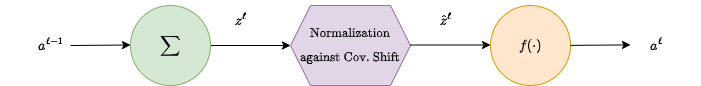
\includegraphics[width=100mm,scale=0.5]{images/nn_2_images/cov_shift_neuron.png}
                
                \caption*{Normalization/standardization can be treated just like any other module.}
            \end{figure}

            \subsecdiv

            Note that this preserves the \orgg{information} in our input data:
            
            \begin{itemize}
                \item If one data point has one feature much larger than another, you'll still see that: the gap will just be shifted over to zero, and normalized.
                
            \end{itemize}

            \miniex Suppose you have some data: $[1,2,\red{100},3,4,5]$. If you standardize, you get

            \begin{equation}
                [-0.458, -0.433, \red{2.04}, -0.408, -0.383, -0.358, ]
            \end{equation}

            The larger data point still stands out above the rest!
            
            We need to be careful of dimensions:\\

            \begin{clarification}
                Normalization relies on the distribution (mean, s.d.) of our \purp{mini-batch}.

                But that means we can't just compute one data point at a time: we need to include the whole mini-batch of $k$ \gren{at the same time}.

                So, we have to change the dimensions of $Z^\ell$.

                $k$ is our \purp{batch size}, while $n$ is the number of \gren{dimensions}. 
                

                \begin{itemize}
                    \item $Z^\ell$ without norm: $(n^\ell \times 1)$
                    \item $Z^\ell$ with norm: $(n^\ell \times \red{k})$
                \end{itemize}

                We use $Z_{ij}^\ell$ to indicate the $\nth{i}$ dimension of the $\nth{j}$ data point.
            \end{clarification}
            

        

        \subsubsection{Post-Normalization: Choose Mean and S.D.}

            Now, we've adjusted it so that our distribution doesn't "drift", based on our training.

            But, now, we've \textbf{restricted} our model:
            
            \begin{itemize}
                \item We don't necessarily want our mean and standard deviation to be 0 and 1: it would be better to be able to \textbf{control} it.
            \end{itemize}
            
            To accomplish this, we'll \textbf{scale} and \textbf{shift} our input. Thus, we're choosing our mean/s.d. in a deliberate way.
            
            \begin{itemize}
                \item Each dimension needs its own mean and standard deviation.
                \item We have $n$ dimensions, and we need one variable to handle mean (or s.d.) for each: we'll need an $(n \times 1)$ vector.\\
            \end{itemize}

            \begin{concept}
                By doing \orgg{normalization}, we've transformed $Z$ into $\overline{Z}$. 
                
                \begin{itemize}
                    \item This "resets" our mean and standard deviation to 0 and 1.
                \end{itemize}

                However, we want to be able to \textbf{control} our mean and standard deviation. To do so, we introduce two new parameters:

                \begin{itemize}
                    \item $G$: An $(n \times 1)$ vector that \purp{scales} each of our dimensions $\overline{Z}_i$, giving our \purp{standard deviations}.
                    \item $B$: An $(n \times 1)$ vector that \gren{shifts} each of our dimensions $\overline{Z}_i$, giving our \gren{means}.
                \end{itemize}

                Thus, we get the true output of \vocab{batch normalization}:

                \begin{equation*}
                    \red{\widehat{Z}_{ik}} = \pur{G_i} * \red{\overline{Z}_{ij}} + \grn{B_i}
                \end{equation*}

            \end{concept}

            \miniex Here's a sample example using a vector $\overline{z}_j$: only considering one, post-normalization data point $j$. 

            \begin{equation}
                \begin{bmatrix}
                    \widehat{Z}_{1j} \\  \widehat{Z}_{2j} \\ \vdots \\ \widehat{Z}_{kj}
                \end{bmatrix}
                =
                \begin{bmatrix}
                    G_{1} \\  G_{2} \\ \vdots \\ G_{k}
                \end{bmatrix}
                *
                \begin{bmatrix}
                    \overline{Z}_{1j} \\  \overline{Z}_{2j} \\ \vdots \\ \overline{Z}_{kj}
                \end{bmatrix}
                +
                \begin{bmatrix}
                    B_{1} \\  B_{2} \\ \vdots \\ B_{k}
                \end{bmatrix}
            \end{equation}

            Where $*$ indicates element-wise multiplication.

            If we include this in our neuron graph, we now have two new modules:

            \begin{figure}[H]
                \centering
                    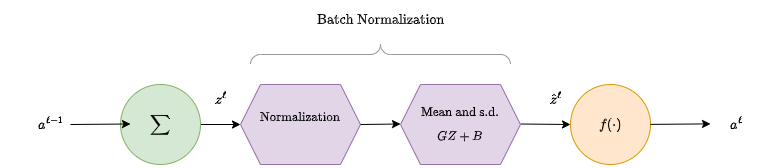
\includegraphics[width=120mm,scale=0.5]{images/nn_2_images/batch_normalization.png}
            \end{figure}

            \subsubsection{Full definition}


            \begin{definition}
                \vocab{Batch Normalization} is a process where we

                \begin{itemize}
                    \item Standardize the pre-activation for each layer using the mean $\mu_i$ and standard deviation $\sigma_i$ (for the $\nth{i}$ dimension). Select $\epsilon$: $0 < \epsilon<<1$.

                    \begin{equation*}
                        \red{ \overline{Z}_{ij} } =  \frac{ \red{Z_{ij}}  -\blu{\mu_i}}{\sigma_i+\epsilon}
                    \end{equation*}
                    
                    \item Choose the new mean and standard deviation for the pre-activation using $(n \times 1)$ vectors $G$ and $B$

                    \begin{equation*}
                        \red{\widehat{Z}_{ik}} = \pur{G_i} * \red{\overline{Z}_{ij}} + \grn{B_i}
                    \end{equation*}
                \end{itemize}

                \subsecdiv

                This process is meant to accomplish the following:

                \begin{itemize}
                    \item Remove possible \purp{internal covariance shift}: training earlier layers may change the scale of inputs to later layers.
                        \begin{itemize}
                            \item This could make training more difficult.
                        \end{itemize}
                    \item Allow our model to \gren{select} a particular mean and s.d. for its pre-activation values, rather than arriving at them by chance.
                \end{itemize}

                It also tends to have a regularizing effect, and, in some learning algorithms, has replaced dropout.
            \end{definition}

        \subsubsection{Effectively Perturbs Data}

            We're not actually sure why normalization helps our models train. We originally designed it for \textbf{internal covariate shift}, but we're not sure if that's really \textbf{why} it works.

            One explanation might be that, due to random sampling, each mini-batch ends up slightly \textbf{modified} by our normalization.
            
            \begin{itemize}
                \item Since each batch is likely to have a slightly different mean/standard deviation, each one ends up differently "perturbed" by normalization.
            \end{itemize}

    \pagebreak
    \subsection{Applying batch normalization to backprop} 

            \phantom{}

            \begin{remark*}
                The following section mostly deals with the details of computing batch normalization derivatives.
            \end{remark*}

            As we showed with our figure,

            \begin{figure}[H]
                \centering
                    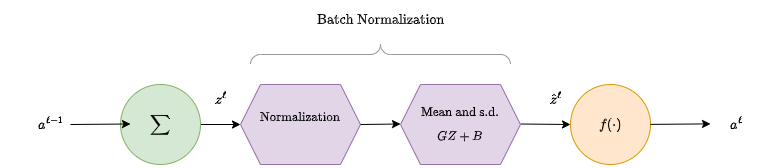
\includegraphics[width=120mm,scale=0.5]{images/nn_2_images/batch_normalization.png}
            \end{figure}

            Batch normalization adds two units that \textbf{interrupt} our chain of nested functions.

            That means we need to figure out how to do backprop, bridging across the new gap between \blu{$Z$} and \red{$\widehat{Z}$}.


            So, that only leaves a couple problems:

            \begin{itemize}
                \item "Bridging the gap" between derivatives before and after BN, with $\pderivslash{\red{\widehat{Z}^\ell}}{\blu{Z^\ell}}$.
                
                \item Gradients for \gren{$G$} and \purp{$B$}: they're parameters now, too, so we need to train them.\\
                
            \end{itemize}

            \begin{concept}
                Introducing batch normalization add new functions \purp{in between} our old ones. 

                \begin{itemize}
                    \item Our input data has to travel through those additional layers.
                    \item This \orgg{changes} the relationship between our current value, and the output loss.
                \end{itemize}

                So, in order to do backprop correctly, we have to figure out the \gren{derivatives} of those functions.
            \end{concept}


        \subsubsection{Bridging the gap}

            We want to connect the start and end of batch normalization:\\

            \begin{equation}
                \pderiv{\red{\widehat{Z}}}{\blu{Z}}
            \end{equation}

            As usual, with the chain rule, we'll connect them by considering any values/function \textbf{between} them.

            In this case, $Z$ is normalized ($\overline{Z}$), and \textbf{then} we apply $G$ and $B$ ($\widehat{Z}$). We're missing the "normalized" step.

            \begin{equation}
                \pderiv{\red{\widehat{Z}}}{\blu{Z}} = 
                \pderiv{\red{\widehat{Z}}}{\grn{\overline{Z}}} \cdot \pderiv{\grn{\overline{Z}}}{\blu{Z}}
            \end{equation}

            Let's compare any two of these : $\red{\widehat{Z}}$ and $\grn{\overline{Z}}$, for example.

            \begin{itemize}
                \item These are both $(n \times k)$ matrices.
                \item That means that each has two dimensions of variables. If we were to take the derivative between them, we would need $2*2$ axes: a \purp{4-tensor}.
            \end{itemize}

            That sounds terrible. Instead, we'll compute these derivatives \textbf{element-wise}.

            \begin{equation}
                \pderiv{ \red{\widehat{Z}_{ab}} }{ \blu{Z_{ef}} } = 
                \pderiv{ \red{\widehat{Z}_{ab}} }{ \grn{\overline{Z}_{cd} } } \cdot 
                \pderiv{ \grn{\overline{Z}_{cd}} }{ \blu{Z_{ef}} }
            \end{equation}

            \subsecdiv

        \subsubsection{Indexing}

            First, let's simplify these indices: only some pairs of elements matter.

            \begin{equation}
                \red{\widehat{Z}_{ik}} = G_i * \grn{\overline{Z}_{ik}} + B_i
            \end{equation}

            It seems that $\red{\widehat{Z}_{ik}}$ is only affected by the element with the same indices: $\grn{\overline{Z}_{ik}}$.\\

            \begin{concept}
                $\red{\widehat{Z}_{ik}}$  is only a function of the same index element $\grn{\overline{Z}_{ik}}$.

                \begin{itemize}
                    \item Any other elements from $\grn{\overline{Z}}$ has no effect.
                \end{itemize}

                \begin{equation*}
                    (\red{a} \neq \grn{c} \text{ or } \red{b} \neq \grn{d}) \implies 
                    \pderiv{ \red{\widehat{Z}_{ab}} }{ \grn{\overline{Z}_{cd} } }=0
                \end{equation*}

                So, we write our remaining derivatives as $\pderivslash{ \red{\widehat{Z}_{ik}} }{ \grn{\overline{Z}_{ik} } }$.
            \end{concept}
        

            What about the other derivative?

            \begin{equation*}
                \grn{ \overline{Z}_{ik} } =  \frac{ \blu{Z_{ik}}  -\blu{\mu_i}}{ \blu{\sigma_i}+\epsilon}
            \end{equation*}

            $\mu_i$ and $\sigma_i$ include various different data points $\blu{Z_{ik}}$, but only the $\nth{i}$ dimension. $\blu{Z_{ik}}$ requires the exact same indices.\\

            \begin{concept}
                $\grn{\overline{Z}_{ik}}$ is only a function of elements in the same dimension $i$, $\blu{Z_{ij}}$.

                \begin{equation*}
                    \grn{c} \neq \blu{e} \implies \pderiv{ \grn{\overline{Z}_{cd}} }{ \blu{Z_{ef}} } = 0
                \end{equation*}

                Our remaining derivatives take the form $\pderivslash{ \grn{\overline{Z}_{ik}} }{ \blu{Z_{ij}} }$.
            \end{concept}

            If we boil this down, we get all of our non-zero derivatives:

            \begin{equation}
                \pderiv{ \red{\widehat{Z}_{ik}} }{ \blu{Z_{ij}} } = 
                \pderiv{ \red{\widehat{Z}_{ik}} }{ \grn{\overline{Z}_{ik} } } \cdot 
                \pderiv{ \grn{\overline{Z}_{ik}} }{ \blu{Z_{ij}} }
            \end{equation}

        \subsubsection{Computing $\pderivslash{ \red{\widehat{Z}_{ik}} }{ \grn{\overline{Z}_{ik} } }$}

            We return to our previous equation:

            \begin{equation}
                \red{\widehat{Z}_{ik}} = G_i * \grn{\overline{Z}_{ik}} + B_i
                \quad \implies \quad
                \pderiv{ \red{\widehat{Z}_{ik}} }{ \grn{\overline{Z}_{ik} } } = G_i
            \end{equation}

        \subsubsection{Computing $\pderivslash{\grn{\overline{Z}_{ik}}}{\blu{Z_{ij}}}$}

            For the other derivative:

            \begin{equation}
                \grn{\overline{Z}_{ik}}  =  \frac{ \org{Z_{ik} }  - \org{\mu_i}}{\org{\sigma_i}+\epsilon}
            \end{equation}

            This gets a bit complicated, because $\blu{Z_{ij}}$ can affect three different terms: $\org{Z_{ik}}$, $\org{\mu_i}$, and $\org{\sigma_i}$. 

            We'll solve this by using the multi-variable chain rule.
                \note{We're linearly adding the effect due to each of these three variables, separately.}

            \begin{equation}
                \pderiv{\grn{\overline{Z}_{ik}}}{\blu{Z_{ij}}} 
                \;\;=\;\;
                \overbrace{
                    \pderiv{\grn{\overline{Z}}_{ik}}{\org{Z_{ik}}} \cdot 
                    \deriv{\org{Z_{ik}}}{\blu{Z_{ij}}}
                }^{\text{$\org{Z_{ik}}$'s effect}}
                \;\;+\;\;
                \overbrace{
                    \pderiv{\grn{\overline{Z}}_{ik}}{\org{\mu_i}} \cdot 
                    \deriv{\org{\mu_i}}{\blu{Z_{ij}}}
                }^{\text{$\org{\mu_i}$'s effect}}
                \;\;+\;\;
                \overbrace{
                    \pderiv{\grn{\overline{Z}}_{ik}}{\org{\sigma_i}} \cdot 
                    \deriv{\org{\sigma_i}}{\blu{Z_{ij}}}
                }^{\text{$\org{\sigma_i}$'s effect}}
            \end{equation}

            In each of these terms, we treat the other two variables as "constant".

        \subsubsection{Lots of mini-derivatives}

            Let's compute the $\grn{\overline{Z}}$ derivatives.

            \begin{equation}
                \grn{\overline{Z}_{ik}}  =  \frac{ Z_{ik}   - \mu_i}{\sigma_i+\epsilon}
            \end{equation}

            gives us

            \begin{equation}
                \pderiv{\grn{\overline{Z}}_{ik}}{\org{Z_{ik}}} = 
                \frac{1}{\sigma_i+\epsilon}
                    \qquad \qquad
                \pderiv{\grn{\overline{Z}}_{ik}}{\org{\mu_i}} = 
                \frac{-1}{\sigma_i+\epsilon}
                    \qquad \qquad
                \pderiv{\grn{\overline{Z}}_{ik}}{\org{\sigma_i}} = 
                -\Big( 
                    \frac{ Z_{ik}-\mu_i  }{(\sigma_i+\epsilon)^2}
                \Big)
            \end{equation}

            Now, let's compute the $\blu{Z_{ij}}$ derivatives.

            \begin{equation}
                \boxed{\pderiv{\org{Z_{ik}}}{\blu{Z_{ij}}} = \delta_{jk}} 
                =
                \mathbf{1}(j=k) = 
                \begin{cases}
                    1 & j=k \\
                    0 & j \neq k
                \end{cases}
            \end{equation}

            \begin{equation}
                \org{\mu_i} =\frac{1}{K} \sum_{j=1}^K \blu{Z_{ij}} 
                    \implies 
                \boxed{\pderiv{ \org{\mu_i} }{ \blu{Z_{ij}} } = \frac{1}{K}}
            \end{equation}

            \begin{equation}
                \org{\sigma^2_i} = \frac{1}{K} \sum_{j=1}^K (\blu{Z_{ij}}-\mu_i)^2  
                    \implies 
                \boxed{\pderiv{ \org{\sigma_i} }{ \blu{Z_{ij}} } = \frac{\blu{Z_{ij}}-\mu_i}{K\sigma_i}}
            \end{equation}

            

            
        \subsubsection{Assembling our derivatives}

            Now, we plug them in.

            \begin{equation}
                \pderiv{\grn{\overline{Z}_{ik}}}{\blu{Z_{ij}}} =
                \pderiv{\grn{\overline{Z}}_{ik}}{\org{Z_{ik}}} \cdot 
                \deriv{\org{Z_{ik}}}{\blu{Z_{ij}}}
                +
                \pderiv{\grn{\overline{Z}}_{ik}}{\org{\mu_i}} \cdot 
                \deriv{\org{\mu_i}}{\blu{Z_{ij}}}
                +
                \pderiv{\grn{\overline{Z}}_{ik}}{\org{\sigma_i}} \cdot 
                \deriv{\org{\sigma_i}}{\blu{Z_{ij}}}
            \end{equation}

            First, the $\grn{\overline{Z}}$ derivatives.

            \begin{equation}
                \pderiv{\grn{\overline{Z}_{ik}}}{\blu{Z_{ij}}} =
                \Big( \frac{1}{\sigma_i+\epsilon} \Big) \cdot 
                \deriv{\org{Z_{ik}}}{\blu{Z_{ij}}}
                -
                \Big( \frac{1}{\sigma_i+\epsilon} \Big) \cdot 
                \deriv{\org{\mu_i}}{\blu{Z_{ij}}}
                -
                \Big( 
                    \frac{ Z_{ik}-\mu_i  }{(\sigma_i+\epsilon)^2}
                \Big) \cdot 
                \deriv{\org{\sigma_i}}{\blu{Z_{ij}}}
            \end{equation}

            And now the $\blu{Z_{ij}}$ derivatives.

            \begin{equation}
                \pderiv{\grn{\overline{Z}_{ik}}}{\blu{Z_{ij}}} =
                \Big( \frac{1}{\sigma_i+\epsilon} \Big) \cdot 
                \delta_{jk}
                -
                \Big( \frac{1}{\sigma_i+\epsilon} \Big) \cdot 
                \Big( \frac{1}{K} \Big)
                -
                \Big( 
                    \frac{ Z_{ik}-\mu_i  }{(\sigma_i+\epsilon)^2}
                \Big) \cdot 
                \Big( \frac{\blu{Z_{ij}}-\mu_i}{K\sigma_i} \Big)
            \end{equation}

            \begin{kequation}
                We have found the batch normalization derivatives

                \begin{equation*}
                    \pderiv{ \red{\widehat{Z}_{ik}} }{ \grn{\overline{Z}_{ik} } } = G_i
                \end{equation*}

                \begin{equation*}
                    \pderiv{\grn{\overline{Z}_{ik}}}{\blu{Z_{ij}}} =
                    \frac{1}{K(\sigma_i+\epsilon)}
                    \Big( K \delta_{jk} - 1 - \frac{(Z_{ik}-\mu_i)(Z_{ij}-\mu_i)}{\sigma_i(\sigma_i+\epsilon)} \Big)
                \end{equation*}

                Which we multiply together to find $\pderivslash{ \red{\widehat{Z}_{ik}} }{ \blu{Z_{ij}} }$.
            \end{kequation}

            Once we've computed these derivatives, we can use them to extend the chain of $\pderivslash{L}{\red{\widehat{Z}_{ik}} }$. 

            We're aiming to handle both of the batch normalization functions, with $\pderivslash{L}{\blu{Z_{ij}}}$. 
                \note{We're going from $\red{\widehat{Z}_{ik}}$, which is post-BN, to $\blu{Z_{ij}}$, which is pre-BN. }

            \begin{itemize}
                \item $\blu{Z_{ij}}$ affects every data point $\red{\widehat{Z}_{ik}}$, and every data point affects $L$.
                \item So, we'll have to consider every data point $k$ using the multi-variable chain rule:
            \end{itemize}
            

            \begin{equation}
                \pderiv{L}{\blu{Z_{ij}}} = 
                \underbrace{ \sum_{k=1}^K }_{\text{MV Chain Rule}}
                \overbrace{
                    \pderiv{L}{\red{\widehat{Z}_{ik}} } \cdot 
                    \pderiv{ \red{\widehat{Z}_{ik}} }{ \blu{Z_{ij}} }
                }^{\text{Data point $k$'s effect}}
            \end{equation}

            We can use this to go further back in our layers: as far as we want, as long as we don't forget this derivative!
            

        \subsubsection{Gradients for $B$ and $G$}

            We want $\pderivslash{L}{\org{B}}$ and $\pderivslash{L}{\pur{G}}$. Thanks to the work we did just now, we can travel backwards through numberous layers, to reach any $B^\ell$ and $G^\ell$. 

            So, we'll assume we have $\pderivslash{L}{\widehat{Z^\ell}}$. Once again, we'll omit the layer notation.

            \begin{itemize}
                \item We'll focus on a single bias, $B_i$: this biases one dimension of $\red{\widehat{Z}_{ik}}$.

                \begin{equation}
                    \red{\widehat{Z}_{ik}} = \pur{G_i} * \grn{\overline{Z}_{ik}} + \org{B_i}
                    \quad \implies \quad
                    \pderiv{ \red{\widehat{Z}_{ik}} }{ \org{B_i} }  = 1
                \end{equation}
                
                \item This bias is applied to every of our $K$ data points: every data point affects the loss $L$. So, we'll have to sum them with the multi-variable chain rule.
            \end{itemize}

            This is exactly the same as how we did $\pderivslash{L}{\blu{Z_{ij}}}$.

            \begin{equation}
                \pderiv{L}{\org{B_i}} = 
                \sum_{k=1}^K 
                \pderiv{L}{ \red{\widehat{Z}_{ik}} } \cdot \pderiv{\red{\widehat{Z}_{ik}}}{\org{B_i}} =
                \boxed{
                \sum_{k=1}^K 
                \pderiv{L}{ \red{\widehat{Z}_{ik}} }
                }
            \end{equation}

            Now, we focus on a single scaling factor $G_i$: 

            \begin{equation}
                \red{\widehat{Z}_{ik}} = \pur{G_i} * \grn{\overline{Z}_{ik}} + \org{B_i}
                \quad \implies \quad
                \pderiv{ \red{\widehat{Z}_{ik}} }{ \pur{G_i}  }  = \grn{\overline{Z}_{ik}}
            \end{equation}

            And once again, we add across different data points:

            \begin{equation}
                \pderiv{ L }{ \pur{G_i}  } = 
                \sum_{k=1}^K 
                \pderiv{L}{ \red{\widehat{Z}_{ik}} } \cdot \pderiv{\red{\widehat{Z}_{ik}}}{\pur{G_i}} =
                \boxed{
                    \sum_{k=1}^K 
                    \pderiv{L}{ \red{\widehat{Z}_{ik}} } \grn{\overline{Z}_{ik}}
                }
            \end{equation}


        We're finished.

        \begin{kequation}
            Here, we have the gradients for the batch scaling coefficients, $B$ and $G$.

            \begin{equation*}
                \pderiv{L}{\org{B_i}} =
                \sum_{k=1}^K 
                \pderiv{L}{ \red{\widehat{Z}_{ik}} }
            \end{equation*}

            \begin{equation*}
                \pderiv{ L }{ \pur{G_i}  } =
                \sum_{k=1}^K 
                \pderiv{L}{ \red{\widehat{Z}_{ik}} } \grn{\overline{Z}_{ik}}
            \end{equation*}
        \end{kequation}

\pagebreak
\section{Terms}
    \subsection*{Section 7-1}

    \begin{itemize}
        \item Neuron (Unit, Node)
        \item Neural Network
        \item Series and Parallel
        \item Linear Component
        \item Weight $w$
        \item Offset (Bias, Threshold) $w_0$
        \item Activation Function $f$
        \item Pre-activation $z$
        \item Activation $a$
        \item Identity Function
        \item Acyclic Networks
        \item Feed-forward Networks
        \item Layer
        \item Fully Connected
        \item Input dimension $m$
        \item Output dimension $n$
        \item Weight Matrix
        \item Offset Matrix
        \item Layer Notation $A^\ell$
        \item Step function
        \item ReLU function
        \item Sigmoid function
        \item Hyperbolic tangent function
        \item Softmax function
    \end{itemize}

    \subsection*{Section 7-1.5}

    
    \begin{itemize}
        \item Forward pass
        \item Back-Propagation
        \item Weight gradient
        \item Matrix Derivative
        \item Partial Derivative
        \item Multivariable Chain Rule
        \item Total Derivative
        \item Size of a matrix
        \item Planar Approximation
        \item Scalar/scalar derivative
        \item Vector/scalar derivative
        \item Scalar/vector derivative
        \item Vector/vector derivative
        
    \end{itemize}

    \subsection*{Section 7-2}

    \begin{itemize}
        \item Mini-batch
        \item Vanishing/Exploding Gradient
        \item Weighted Average
        \item Running Average
        \item Exponential Moving Average
        \item Discount Factor
        \item Momentum
        \item Adadelta
        \item Adagrad (Optional)
        \item Adam
        \item Normalization
        \item Early stopping (Review)
        \item Weight Decay
        \item Perturbation
        \item Dropout
        \item Covariate Shift
        \item Internal Covariate Shift
        \item Batch Normalization
        \item Multivariable Chain Rule (Review)
    \end{itemize}
            

            
        
        
        
        
        



%%% Local Variables:
%%% mode: latex
%%% TeX-master: "top"
%%% End:
